\chapter{Application: SASI Toy Problem}
\label{chap:application}

As mentioned at the beginning of Chapter~\ref{chap:introduction}, the simple toy model of F09~\cite{Foglizzo2009} and SFF09~\cite{Sato2009} was chosen as a useful initial application of our well-balanced method to the SASI. The salient details from those papers are reproduced here.

The basic set-up of the problem consists of a 2D domain with periodic boundary conditions on both edges in the $x$-direction and three distinct flow regions in the $y$-direction. First is a supersonic inflow, which is transitioned by a shock front at $y=y_\textrm{sh}$ to subsonic speeds in the second region. This is then separated from a third region (also subsonic) by a potential step at $y=y_\nabla$ which further decelerates the flow and provides a simple model of matter slowing as it nears the surface of the accreting object. Following the notation of SFF09, we will denote quantities in the supersonic region before the shock with a subscript `1', in the interior region between the shock and potential step with `in', and in the outflow region past the step with `out'.

A schematic view of the problem domain with all three regions can be seen on the left side of Fig.~\ref{fig:Sato1}, with the right side showing how the overall scenario is then split into two sub-problems for initial simulation. This separation greatly simplifies the introduction of specific advective and acoustic perturbations to appropriate locations in the interior of the domain, making it much easier to see the interactions of these disturbances at the boundaries (the shock and potential step) between the various flow regions. Overall, this provides a much simplified analogue for simulations to study the mechanisms at play during the inflow, decceleration, and accretion of matter in a collapsing star before supernova.

\begin{figure}
\centering
\includegraphics[width=13cm]{figures/Sato1}
\caption {This image is taken directly from SFF09~\cite{Sato2009}. On the left is a schematic diagram of the full toy problem for the SASI,  which is then broken into two sub-problems on the right. Circular arrows represent advective vorticity waves while wavy arrows denote acoustic pressure waves. The coupling efficiencies denote the strength of coupling between acoustic and advective waves ($Q_\textrm{sh}$, $Q_\nabla$) and the reflection of purely acoustic waves ($R_\textrm{sh}$, $R_\nabla$).}
\label{fig:Sato1}
\end{figure}

General parameters of the model problem will be presented next, followed by specific information for the potential step and stationary shock, computed separately as sub-problems 1 and 2, respectively. 


\section{Problem Set-up}
\label{sec:TP_set_up}

The general flow problem to be studied is essentially a 1D flow when at equilibrium, with the periodicity in the $x$-direction mimicking an infinitely wide flow and all variation occuring in the $y$-direction. Simulating this problem in 2D then, is done purely for studying the perturbations to this equilibrium flow, thus allowing more interesting perturbations and potential higher-dimenensional features to also be realized.

An ideal gas with an adiabatic constant $\gamma=4/3$ was simulated, the extent of the domain in the $x$-direction is denoted as $L_x$, and the entropy of the fluid is defined as
\begin{equation}
S\equiv\frac{\log\left(p/\rho^\gamma\right)}{\gamma-1}.
\end{equation}
Beginning with a Mach number of $\mathcal{M}_1=5$ at the inflow, one can then compute the relations of flow values across the shock as defined by the Rankine-Hugoniot conditions
\begin{equation}
\mathcal{M}_\textrm{in}=\sqrt{\frac{2+(\gamma-1)\mathcal{M}_1^2}{2\gamma\mathcal{M}_1^2-\gamma+1}},
\end{equation}
\begin{equation}
\frac{v_1}{v_\textrm{in}}=\frac{(\gamma+1)\mathcal{M}_1^2}{2+(\gamma-1)\mathcal{M}_1^2},
\end{equation}
\begin{equation}
\frac{\rho_1}{\rho_\textrm{in}}=\frac{v_\textrm{in}}{v_1},
\end{equation}
where $v_\textrm{in}=-\mathcal{M}_\textrm{in}c_\textrm{in}$ and the interior Mach number is found to be $\mathcal{M}_\textrm{in}=\sqrt{31/199}\approx0.39$.

A hyperbolic tangent function is used to provide a smooth step-like external potential field centred at $y_\nabla=0$ extant over an approximate width $H_\nabla$, with the exact function given by
\begin{equation}
\phi(y)=\frac{\Delta\phi}{2}\left[\tanh\left(\frac{y-y_{\nabla}}{H_{\nabla}/2}\right)+1\right],
\end{equation}
where the step size $\Delta\phi$ is set based on the ratio of the sound speeds $c_{\textrm{in}}/c_{\textrm{out}}$ in the constant regions surrounding the step, and can be computed as
\begin{equation}
\Delta\Phi=\left(\frac{\mathcal{M}_\textrm{out}^2}{2}+\frac{1}{\gamma-1}\right)c_\textrm{out}^2-\left(\frac{\mathcal{M}_\textrm{in}^2}{2}+\frac{1}{\gamma-1}\right)c_\textrm{in}^2.
\end{equation}
For all simulations, the ratio $c_\textrm{in}^2/c_\textrm{out}^2=0.75$ was used, and the step width was chosen such that $H_\nabla/H=0.1$ where $H\equiv y_\textrm{sh}-y_\nabla$ is defined to be the distance between the shock and the middle of the potential step.

A reference timescale for the advective-acoustic cycle is used to normalize the simulation times, and is calculated as
\begin{equation}
\tau_\textrm{aac}\equiv\frac{1}{1-\mathcal{M}_\textrm{in}}\frac{H}{|v_\textrm{in}|}.
\end{equation}
Units for all quantities are chosen to ensure that $c_\textrm{in}=\rho_\textrm{in}=H=1$. Using the relation $p=\rho c^2/\gamma$ we can compute the other primitive values in the interior region as $p_\textrm{in}=0.75$ and $T_\textrm{in}=1.05$ and the reference timescale as $\tau_\textrm{aac}\approx4.2$. A wavenumber $k_x=2\pi/L_x$ is used to define linear perturbations of the flow, where $L_x=4$, along with a temporal frequency defined as $\omega_0=4\pi/\tau_\textrm{aac}$.

For both sub-problems a $4\times4$ square domain is used, divided into a uniform number $N_x=N_y=400$ of square grid cells in both dimensions. This gives a uniform grid spacing of $\Delta x=\Delta y=10^{-2}$.

\subsection{Sub-Problem 1: Potential Step}
\label{subsec:sub_problem_1}

For the first sub-problem, the potential step positioned at $y_\nabla=0$ is the only flow feature simulated on a square domain defined on $y\in[-1,3]$, $x\in[0,4]$. Inflow occurs at the upper $y=3$ boundary, defined using Dirichlet conditions, and zero-gradient conditions are imposed at the $y=-1$ outflow boundary. Initial conditions are determined by computing the equilibrium flow for the given inlet primitive values over the potential field. By defining also a vertical wavenumber $k_y=\omega_0/v_\textrm{in}$ the perturbations injected at the inlet are given by the equations
\begin{equation}
\delta S\equiv\epsilon_S\cos\left(-\omega_0t+k_xx+k_yy\right),
\end{equation}
\begin{equation}
\frac{\delta \rho}{\rho_\textrm{in}}\equiv\exp\left(-\frac{\gamma-1}{\gamma}\delta S\right)-1,
\end{equation}
where $\epsilon_S=10^{-3}$ is the amplitude of the generated entropy waves.

These incoming waves are desired to be at pressure equilibrium ($\delta p=0$), and so from the equation of state one can then determine the consistent temperature perturbation
\begin{equation}
\frac{\delta T}{T_\textrm{in}}=\left(1+\frac{\delta\rho}{\rho_\textrm{in}}\right)^{-1}-1=\exp\left(\frac{\gamma-1}{\gamma}\delta S\right)-1.
\end{equation}
Deviations to the 2D velocity components are given as
\begin{equation}
\delta v_x\equiv\frac{k_x\omega_0c_\textrm{in}^2}{\omega_0^2+k_x^2v_\textrm{in}^2}\frac{\delta S}{\gamma} \quad \textrm{and} \quad \delta v_y\equiv-\frac{k_x^2v_\textrm{in}c_\textrm{in}^2}{\omega_0^2+k_x^2v_\textrm{in}^2}\frac{\delta S}{\gamma},
\end{equation}
which result in the generation of the following vorticity waves 
\begin{equation}
\delta w_y=-\frac{k_xc_\textrm{in}^2}{v_\textrm{in}}\frac{\epsilon_S}{\gamma}\sin\left(-\omega_0t+k_xx+k_yy\right).
\end{equation}
These waves, which are injected only at the inlet, are allowed to travel through the interior region towards the potential step, and then any resultant coupling of the vorticity waves into reflected pressure waves is observed.

\subsection{Sub-Problem 2: Standing Shock}
\label{subsec:sub_problem_2}

For the second sub-problem, only the shock front positioned at $y_\textrm{sh}=1$ is simulated, with the square domain now defined on $y\in[-2,2]$, $x\in[0,4]$. Inflow is now supersonic and again set with Dirichlet boundaries at $y=2$, although the outflow conditions at $y=-2$ are different from sub-problem 1. Homogoneous Neumann conditions are still used initially while no perturbations are present in the system, to allow the shock to ``settle in'' and any waves generated by this settling process to propagate cleanly out of the system. Once a steady state is reached, however, the outflow conditions are changed to be also Dirichlet in order to inject the desired perturbations into the domain from the outflow boundary. The time at which this ``switching on'' of the injected perturbations occurs is labeled as the starting time $\tau=0$ for the simulations. Initial conditions are in this case determined purely by the Rankine-Hugoniot conditions given earlier to define the shock, since the potential field is now constant throughout the entire domain.

Vorticity-free pressure perturbations are generated for this sub-problem, and by defining a new vertical wavenumber
\begin{equation}
k_y^\pm=\frac{\omega_0}{c_\textrm{in}}\frac{\mathcal{M}_\textrm{in}\mp\mu}{1-\mathcal{M}_\textrm{in}^2},
\end{equation}
and density perturbation amplitude $\epsilon_\rho=10^{-3}$, one has the equations for the perturbations injected at the outlet as
\begin{align}
\frac{\delta\rho}{\rho_\textrm{in}}&\equiv\left(\frac{1+\mu\mathcal{M}_\textrm{in}}{1-\mathcal{M}_\textrm{in}^2}\right)\epsilon_\rho\cos\left(-\omega_0t+k_xx+k_y^-y\right), \\
\frac{\delta p}{p_\textrm{in}}&\equiv\left(1+\frac{\delta\rho}{\rho_\textrm{in}}\right)^\gamma-1,
\end{align}
where one can again use the equation of state to determine the consistent temperature deviation
\begin{equation}
\frac{\delta T}{T_\textrm{in}}=\left(1+\frac{\delta\rho}{\rho_\textrm{in}}\right)^{\gamma-1}-1.
\end{equation}
Velocity perturbations for these purely acoustic pressure waves are given by
\begin{align}
\delta v_x&\equiv\left(\frac{k_xc_\textrm{in}^2}{\omega_0}\right)\epsilon_\rho\cos\left(-\omega_0t+k_xx+k_y^-y\right), \\
\delta v_y&\equiv\left(\frac{\mu+\mathcal{M}_\textrm{in}}{1-\mathcal{M}_\textrm{in}^2}\right)c_\textrm{in}\epsilon_\rho\cos\left(-\omega_0t+k_xx+k_y^-y\right),
\end{align}
where the parameter $\mu$ is simply used for convenience and expands as
\begin{equation}
\mu\equiv\sqrt{1-\frac{k_x^2c_\textrm{in}^2}{\omega_0^2}\left(1-\mathcal{M}_\textrm{in}^2\right)}.
\end{equation}
These waves then propagate towards the shock front, and any resultant generation of reflected vorticity waves is measured.


\section{Numerical Results}
\label{sec:TP_results}

Results of simulations for the two sub-problems are presented next, comparing the results to those obtained in F09 and SFF09.

\subsection{Sub-Problem 1}
\label{subsec:results_TP1}

In Fig.~\ref{fig:TP1} can be seen the numerical results obtained for the potential step problem using the well-balanced scheme, with data presented in a manner similar to Fig.~2 in SFF09 to allow easy comparison. At three successive times, the first before and the second and third after the injected entropy/vorticity waves have reached the potential step, are shown the specific vorticity on the left and the normalized pressure perturbation on the right. Excellent qualitative agreement is seen to the corresponding figure in SFF09. Before the incident wave reaches the step, the right hand column is largely free of any perturbations, with reflected and (less strong) transmitted pressure deviations observed only as the incident wave passes through the deceleration zone centred at $y_\nabla=0$, illustrating clear generation of acoustic waves as the incoming vorticity wave is decelerated at the potential step. It is also clear to see that in comparison to the figure in SFF09, there is essentially no spurious deviation from the equilibrium flow observed over the potential step itself in our simulation with the new well-balanced scheme, at any of the timepoints.

\begin{figure}
\centering
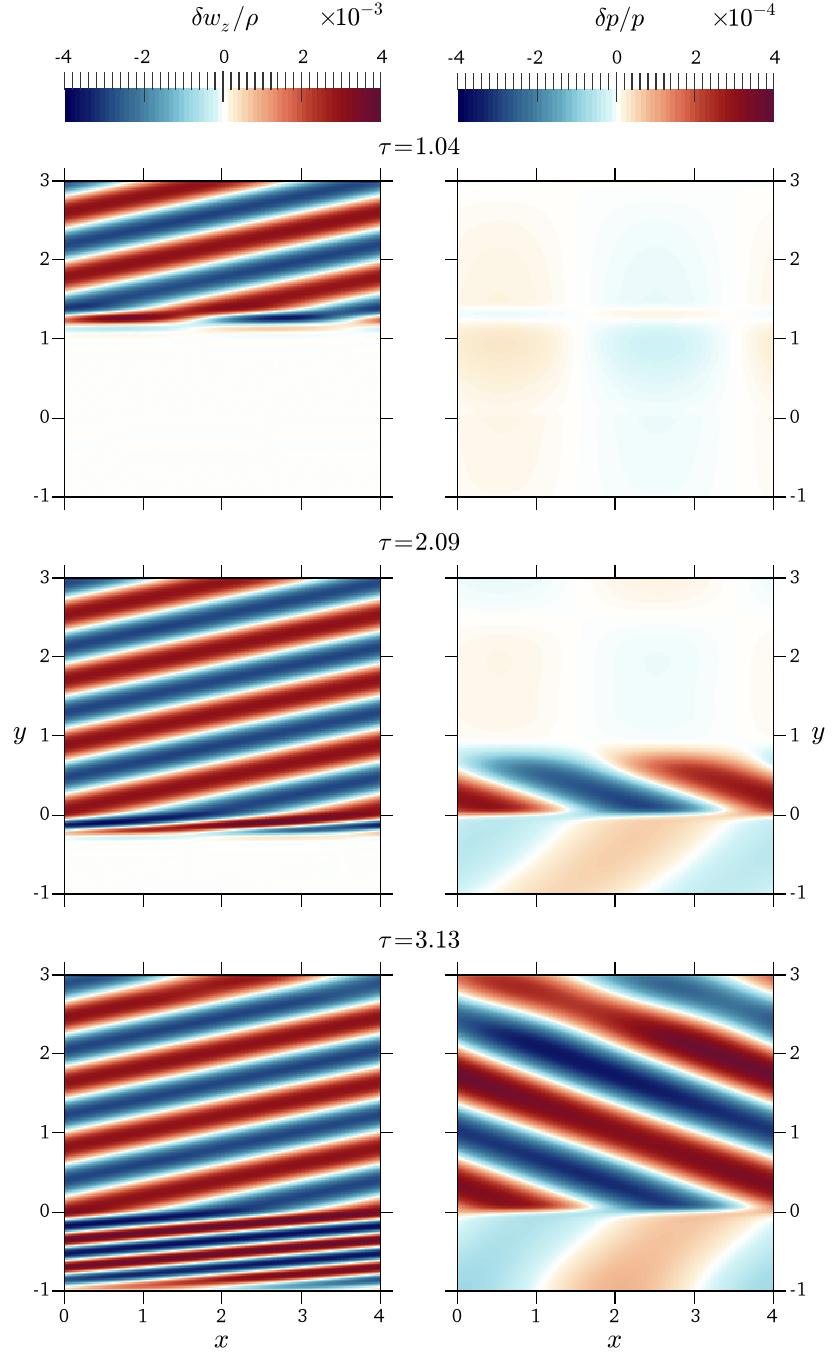
\includegraphics[width=12cm]{figures/TP1}
\caption {Results of sub-problem 1 which can be compared to Fig.~2 in SFF09~\cite{Sato2009}. Generation of an acoustic wave by the deceleration of a vorticity wave through a potential step centred at $y_\nabla=0$ is shown at three successive times $\tau$, normalized by $\tau_\textrm{aac}$.}
\label{fig:TP1}
\end{figure}

In order to obtain a more quantitative comparison, the amplitude of the acoustic feedback was measured, using a Fourier transform of the induced pressure perturbation, over one full wave period $T\equiv2\pi/\omega_0$, with the transform defined by
\begin{equation}
\hat{\delta p}_0=\frac{2}{T}\int\limits_{0}^{T}\delta pe^{i\omega_0t}\textrm{d}t.
\end{equation}
By assuming that the generated acoustic wave is advected away from the potential step relatively unchanged, in essence invoking Taylor's frozen turbulence hypothesis, the data for the perturbation was taken from the final timepoint ($\tau=3.13$) by measuring over a full spatial wavelength. These values are then cast back to the time domain by pairing the datapoints with the correct Fourier frequencies for the integration, as if they had in fact been taken at a single spatial point over the above time interval. With this, the efficiency of the acoustic feedback from the incoming entropy wave is calculated to be $$\left(\hat{\delta p}_0/p_\textrm{in}\right)/\delta S=0.338.$$
In order to have a good value for comparison, the expected value was read off the analytic solution line of Fig.~3 in SFF09 for the simulated frequency of $\omega_0\tau_\textrm{aac}/2\pi=2$ and determined to be approximately $\left(\hat{\delta p}_0/p_\textrm{in}\right)/\delta S=0.32$. This therefore shows excellent agreement between our simulated results and the expected value from the linear analysis undertaken in F09.

\subsection{Sub-Problem 2}
\label{subsec:results_TP2}

For the standing shock sub-problem, the results of the well-balanced simulation are shown in Fig.~\ref{fig:TP2}, here presented to allow easy comparison with Fig.~4 in SFF09. Data is again shown for three successive timepoints, in this instance before and after a pressure wave, injected at the outflow, reaches the shock front. Once there, it produces coupled vorticity/entropy perturbations back into the interior region, with excellent qualitative agreement for the advective-acoustic wave cycling observed with the respective figure in SFF09.

While there are a few very small spurious deviations visible in the specific vorticity (shown in the left hand column of the figure) in the immediate vicinity of the the shock throughout the simulation, the domain is predominantly vorticity-free before the incident wave reaches the shock. Only after the pressure wave, visible in the normalized pressure deviation shown in the right hand column of the figure, impacts the shock is clear generation of advective waves observed. This provides evidence for the necessary second half of the advective-acoustic cycle, complementing the generation of vorticity waves from incident pressure waves at the potential step observed in sub-problem 1.

\begin{figure}
\centering
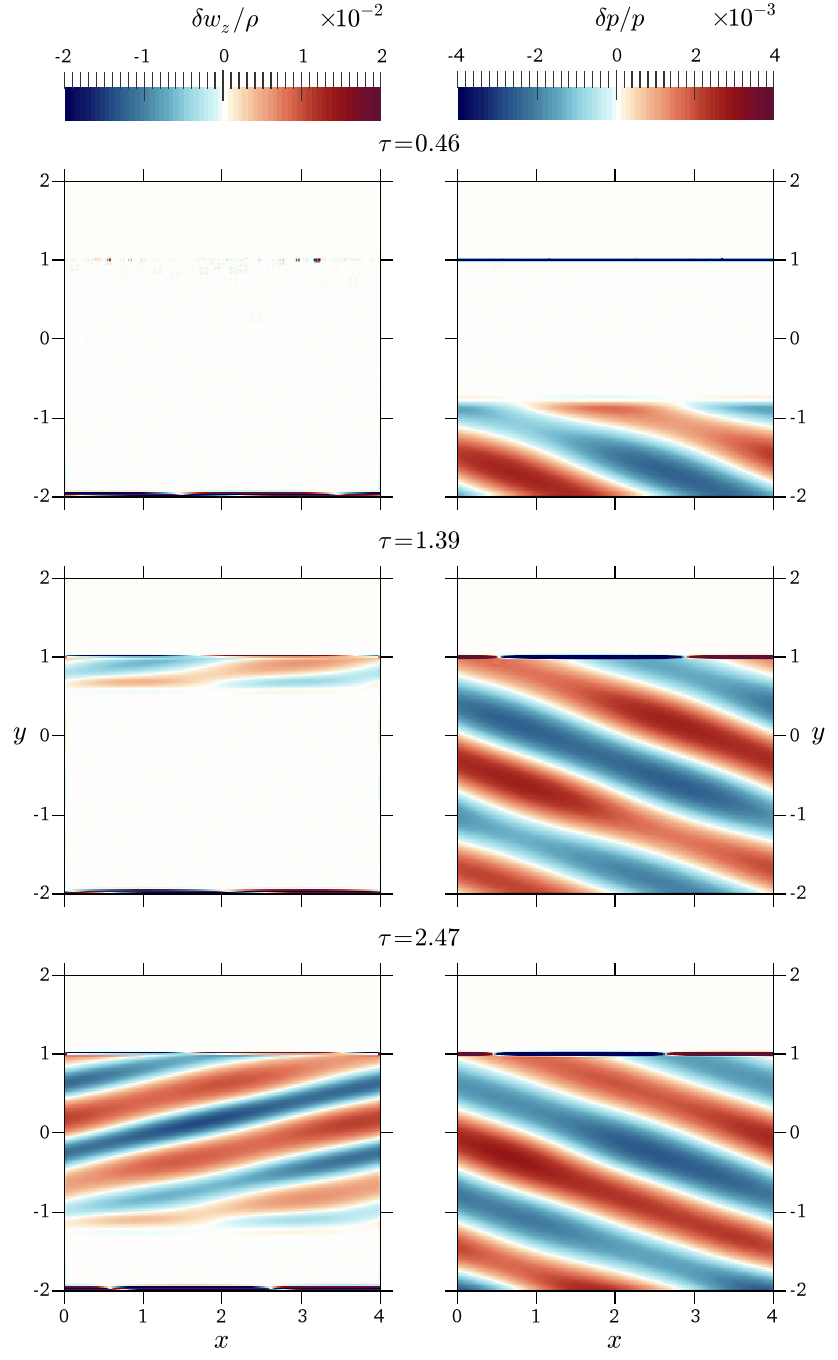
\includegraphics[width=12cm]{figures/TP2}
\caption {Results of sub-problem 2 which can be compared to Fig.~4 in SFF09~\cite{Sato2009}. Generation of a vorticity wave by the reflection of an acoustic wave from a shock located at $y_{\textrm{sh}}=1$ is shown at three successive times $\tau$, normalized by $\tau_\textrm{aac}$.}
\label{fig:TP2}
\end{figure}

To once again have a more quantitative check of the results in addition to the qualitative agreement with SFF09 observed above, the amplitude of the resulting entropy wave was measured for comparison to the expected value from theory. This theoretical value can be computed directly according to the formula from SFF09
\begin{equation}
\delta S_\textrm{th}=\frac{\delta p}{p_\textrm{in}}\frac{2}{\mathcal{M}_\textrm{in}}\frac{1-\mathcal{M}_\textrm{in}^2}{1+\gamma\mathcal{M}_\textrm{in}^2}\left(1-\frac{\mathcal{M}_\textrm{in}^2}{\mathcal{M}_1^2}\right)\frac{\mu}{\mu^2+2\mu\mathcal{M}_\textrm{in}+\mathcal{M}_1^{-2}},
\end{equation}
and for the given simulation is found to be $\delta S_\textrm{th}=3.28\textrm{e-}3$.

Analyzing the results of the numerical simulation at the final timetep from the figure, $\tau=2.47$, the amplitude of the generated entropy wave is measured to be $$\delta S_\textrm{sim}=2.94\textrm{e-}3.$$ This once again demonstrates relatively good agreement between the results obtained using the newly implemented well-balanced method and the theoretically expected value determined from the analytic treatment of F09 and SFF09.

With both parts of the advective-acoustic cycle thus independently observed, it remains to then put the two sub-problems together for a simulation of both effects concurrently.

\subsection{Full Toy Problem}
\label{subsec:results_TP}

The complete toy problem was simulated, with both the standing shock and the potential step now present in the domain simultaneously. Perturbations to the density and pressure equilibria were introduced in the supersonic inflow region to mimic spatial inhomogeneities which could be present in the distribution of accreting matter prior to a core-collapse supernova.

Keeping the same horizontal wavenumber $k_x=2\pi/L_x$ but defining a new vertical wavenumber as $k_y=\omega_0/v_1$ and density perturbation amplitude as $\epsilon_\rho=10^{-4}$ we have the following equations for the density and pressure perturbations at the supersonic inflow
\begin{equation}
\delta\rho=\epsilon_\rho\cos\left(-\omega_0t+k_xx+k_yy\right),
\end{equation}
\begin{equation}
p=p_1+\delta p=(\rho_1+\delta\rho)RT_1,
\end{equation}
where $R$ is the specific gas constant and the velocity and temperature are kept at constant equilibrium ($\delta v=\delta T=0$).

Initial conditions were set by splicing together the ``settled in'' initial conditions used for the shock in sub-problem 2 with the analytically computed equlibrium used for the sub-problem 1 initial conditions, with the join occuring just below the shock at $y=0.92$. For all quantities Dirichlet boundary conditions were imposed at the inlet with homogenous Neumann conditions used at the outflow.

The simulation was allowed to progress to a final time of $\tau=3$ (normalized by $\tau_{aac}$) where the time origin $\tau=0$ was set to be the time just before the incoming perturbations impacted on the shock front. Measurements of the maximal perturbation amplitudes were taken in the interior region between the shock and the potential step, $y\in[0.1,0.9]$, and these values are tabulated in Table~\ref{table:TP} for several key timepoints. Visual results for three of these timepoints are also shown in Fig.~\ref{fig:TP} for comparison.

\begin{table*}\centering
\caption{Maximum amplitudes of the specific advective and acoustic perturbations in the interior region between the shock and potential step at successive times $\tau$, normalized by $\tau_\textrm{aac}$.}
\ra{1.3}
\label{table:TP}
\begin{tabular}{@{}lcccc@{}}\toprule
& \phantom{abc} & \multicolumn{3}{c}{Perturbation Amplitude} \\
\cmidrule{3-5}
\phantom{al}$\tau$ && $\delta w_z/\rho$ & \phantom{abc} & $\delta p/p$ \\
\midrule
$0.125$ && 2.99e-03 && 2.83e-04 \\
$0.500$ && 3.23e-03 && 4.01e-04 \\
$1.00$ && 3.65e-03 && 6.65e-04 \\
$2.00$ && 5.21e-03 && 8.12e-04 \\
$3.00$ && 5.95e-03 && 8.89e-04 \\
\bottomrule
\end{tabular}
\end{table*}

\begin{figure}
\centering
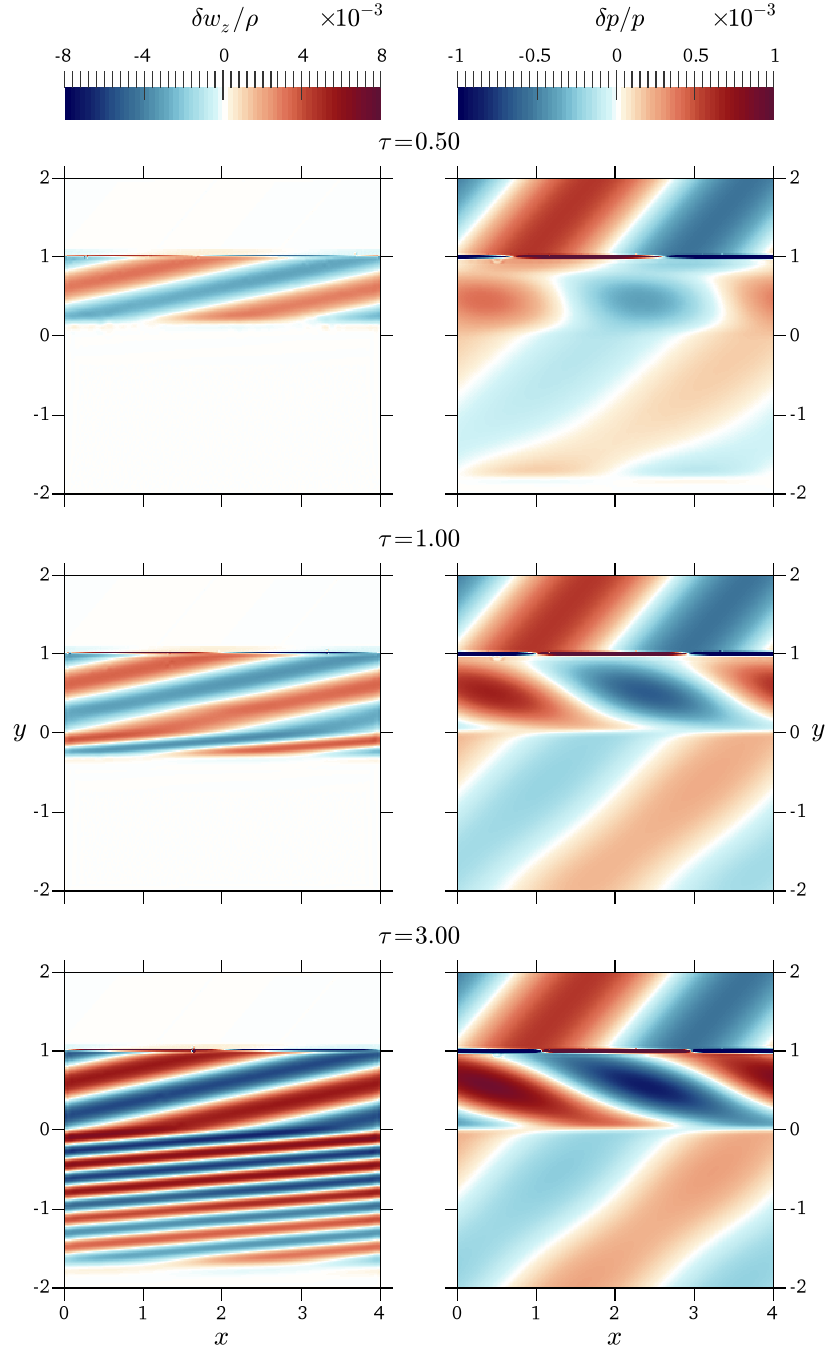
\includegraphics[width=12cm]{figures/TP}
\caption {Results of the full toy problem simulation, showing the advective-acoustic cycle. Coupling of vorticity and pressure waves at both a shock located at $y_{\textrm{sh}}=1$ and a potential step located at $y_\nabla=0$ is shown at three successive times $\tau$, normalized by $\tau_\textrm{aac}$.}
\label{fig:TP}
\end{figure}

At the first time given in the table, $\tau=0.125$ (not shown in figure), the incident perturbations have reached the shock and resultant perturbations in both the pressure and vorticity are observed being generated and travelling into the interior region. Neither of these wave types have yet reached the potential step at this point, and so the amplitudes given in the table represent purely the strength of the coupling from the injected perturbations in the supersonic inflow.

Moving to the second time in the table, $\tau=0.5$ (top row of figure), the faster moving acoustic wave has now reached the potential step, with part of the energy being transmitted through to the outflow and part reflected back into the interior, with the amplitude for the specific pressure perturbation observed to increase noticeably. By contrast, the slower moving advective wave has not yet reached the potential step, and no coupling of acoustic to advective waves is observed at the potential step, and so the measured amplitude of the specific vorticity perturbations has not increased by much from the initial value.

At $\tau=1$ (middle row of figure), the advective wave has now also reached the potential step, and coupled reflection of acoustic waves back into the interior region is observed, and is evidenced by another significant increase in the measured amplitude of the specific pressure deviation. No reflection of these advective perturbations is observed, of course, but some transmission of vorticity into the outflow can be clearly seen. A small increase in the specific vorticity perturbation amplitude is measured, due to the coupling at the shock of the acoustic reflections from the potential step noted previously at $\tau=0.5$, but the much larger coupled acoustic waves generated from the advective waves impacting on the potential step have not quite reached the shock at this time.

For the final times represented in the table, $\tau=2$ (not shown in figure) and $\tau=3$ (bottom row of figure), the acoustic waves generated by advective coupling at the potential step have now reached the shock and themselves coupled to produce further vorticity perturbations in the interior region, thus completing the full advective-acoustic cycle. This is evidenced by the much more significant increase in the specific vorticity perturbation amplitude compared to the previous time point. Through these final times simulated, the amplitudes for both types of waves continue to rise as further perturbation energy is deposited into the advective-acoustic cycle that is now established between the shock and and the potential step.